\documentclass[a4paper,12pt]{book}

\usepackage[T1]{fontenc}
\usepackage[T2A]{fontenc}
\usepackage[utf8x]{inputenc}
\usepackage[russian]{babel}
\usepackage{geometry}
\usepackage{graphicx}
\usepackage{amssymb}

\geometry{left=1.5cm}
\geometry{right=2.5cm}
\geometry{top=0.7cm}
\geometry{bottom=2cm}

\begin{document}
\fontsize{14pt}{14pt}\selectfont
\parindent=0.0cm
{\small 20.5 \textit{Геометрический смысл частных производных и дифференциала}\ \ \ \ \ \ \ \ \ \ \ \ \ \ \ \ \ \ \ \ \ \ \ \ \ \ \ \ \ \ \ \ \ \ 303}\par
\vspace{1.5em}
\parindent=0.7cm
Рассмотрим функцию $z=f(x, y)$, определенную на плоском открытом множестве $G$, т. е. множестве $G$, лежащем на плоскости $E^2$.\par
\parindent=0.0cm
Пусть $(x_0,y_0) \in G$ и пусть в точке $(x_0,y_0)$ существует частная производная $\frac{\partial z}{\partial x}$. Ее геометрический смысл сразу получается из определения частной производной $\frac{\partial z}{\partial x}$ как обычной производной функции\par
\begin{center}
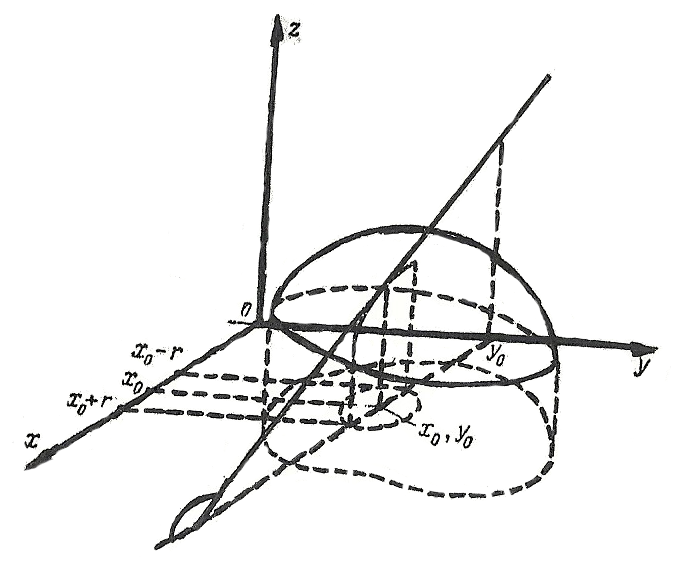
\includegraphics[scale=1.5]{grafik.png}\par
{\small \textit{Рис}. 74}\par
\end{center}
$f(x,y)$ по $x$ при фиксированном $y$ и из геометрического смысла обычной производной (см. п. 9.3). В самом деле, возьмем замкнутый круг $Q$ радиуса $r$ с центром в точке $(x_0,y_0)$ и лежащий в $G^{*)}$. Пусть $\gamma$ - кривая, заданная представлением\par
$$
z=f(x_0,y_0)
$$\par
$$
y=y_0
$$\par
$$
x_0-r \leqslant x \leqslant x_0+r,
$$\par
т. е. кривая, которая получается сечением графика функции $z=f(x,y), (x,y) \\
\in Q$ плоскостью $y=y_0$ (рис. 74).\par
\line(1,0){64}\par
\parindent=0.7cm
{\small *) Такой круг $Q$ всегда существует. Действительно, в силу определения открытого множества существует такая $\delta$ - окрестность $O$ точки $(x_0,y_0)$, что $O \subset G$. Тогда замкнутый круг $Q$ радиуса $\frac{\delta}{2}$ с центром в точке $(x_0,y_0)$ будет заведомо лежать в $G$.
}
\end{document}
